% TikZ Figure: Hierarchical Graph Allocation & Layer Decoupling
% Illustrates Upper Layer Long-Range Highways vs Layer 0 Geometric Degree Allocation
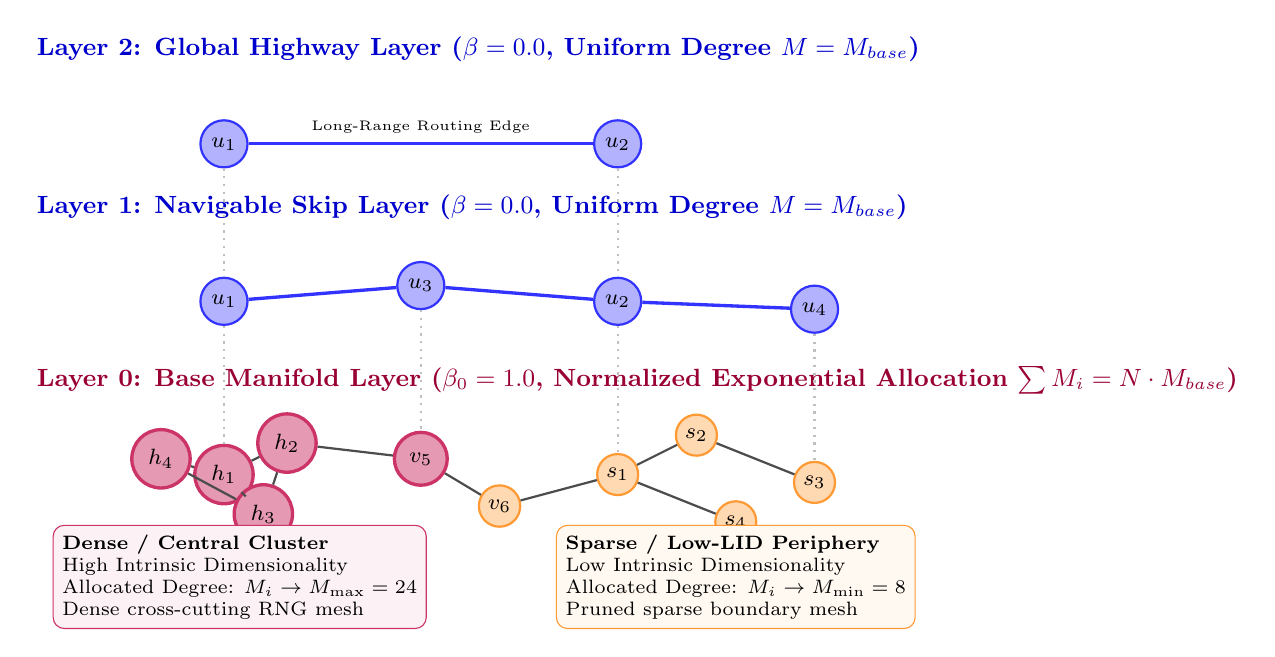
\begin{tikzpicture}[
    font=\sffamily\footnotesize,
    layerbox/.style={draw=black!60, fill=gray!5, dashed, rounded corners=6pt, inner sep=10pt},
    nodeUpper/.style={circle, draw=blue!80, fill=blue!30, thick, inner sep=2.5pt},
    nodeL0Dense/.style={circle, draw=purple!80, fill=purple!40, very thick, inner sep=3.5pt},
    nodeL0Sparse/.style={circle, draw=orange!80, fill=orange!30, thick, inner sep=2pt},
    edgeUpper/.style={draw=blue!80, very thick},
    edgeL0/.style={draw=black!70, thick},
    projEdge/.style={draw=gray!50, dotted, thick}
]

% Layer 2 (Top Highway)
\begin{scope}[yshift=4.2cm]
    \node[anchor=west, font=\bfseries\small, text=blue!80!black] at (-0.5, 1.2) {Layer 2: Global Highway Layer ($\beta = 0.0$, Uniform Degree $M=M_{\text{base}}$)};
    \node[nodeUpper] (l2_1) at (2.0, 0.0) {$u_1$};
    \node[nodeUpper] (l2_2) at (7.0, 0.0) {$u_2$};
    \draw[edgeUpper] (l2_1) -- (l2_2) node[midway, above, font=\tiny] {Long-Range Routing Edge};
\end{scope}

% Layer 1 (Intermediate Skip Layer)
\begin{scope}[yshift=2.2cm]
    \node[anchor=west, font=\bfseries\small, text=blue!80!black] at (-0.5, 1.2) {Layer 1: Navigable Skip Layer ($\beta = 0.0$, Uniform Degree $M=M_{\text{base}}$)};
    \node[nodeUpper] (l1_1) at (2.0, 0.0) {$u_1$};
    \node[nodeUpper] (l1_2) at (4.5, 0.2) {$u_3$};
    \node[nodeUpper] (l1_3) at (7.0, 0.0) {$u_2$};
    \node[nodeUpper] (l1_4) at (9.5, -0.1) {$u_4$};
    \draw[edgeUpper] (l1_1) -- (l1_2);
    \draw[edgeUpper] (l1_2) -- (l1_3);
    \draw[edgeUpper] (l1_3) -- (l1_4);
\end{scope}

% Layer 0 (Base Graph with Geometry-Aware Degrees)
\begin{scope}[yshift=0.0cm]
    \node[anchor=west, font=\bfseries\small, text=purple!80!black] at (-0.5, 1.2) {Layer 0: Base Manifold Layer ($\beta_0 = 1.0$, Normalized Exponential Allocation $\sum M_i = N \cdot M_{\text{base}}$)};
    % High-density cluster (Hubs)
    \node[nodeL0Dense] (l0_1) at (2.0, 0.0) {$h_1$};
    \node[nodeL0Dense] (l0_2) at (2.8, 0.4) {$h_2$};
    \node[nodeL0Dense] (l0_3) at (2.5, -0.5) {$h_3$};
    \node[nodeL0Dense] (l0_4) at (1.2, 0.2) {$h_4$};
    
    % Dense cluster interconnects (High M, up to M_max = 24)
    \draw[edgeL0] (l0_1) -- (l0_2);
    \draw[edgeL0] (l0_1) -- (l0_3);
    \draw[edgeL0] (l0_1) -- (l0_4);
    \draw[edgeL0] (l0_2) -- (l0_3);
    \draw[edgeL0] (l0_4) -- (l0_3);
    
    % Intermediate transit nodes
    \node[nodeL0Dense] (l0_5) at (4.5, 0.2) {$v_5$};
    \node[nodeL0Sparse] (l0_6) at (5.5, -0.4) {$v_6$};
    \draw[edgeL0] (l0_2) -- (l0_5);
    \draw[edgeL0] (l0_5) -- (l0_6);
    
    % Sparse peripheral manifold (Low M, down to M_min = 8)
    \node[nodeL0Sparse] (l0_7) at (7.0, 0.0) {$s_1$};
    \node[nodeL0Sparse] (l0_8) at (8.0, 0.5) {$s_2$};
    \node[nodeL0Sparse] (l0_9) at (9.5, -0.1) {$s_3$};
    \node[nodeL0Sparse] (l0_10) at (8.5, -0.6) {$s_4$};
    \draw[edgeL0] (l0_6) -- (l0_7);
    \draw[edgeL0] (l0_7) -- (l0_8);
    \draw[edgeL0] (l0_8) -- (l0_9);
    \draw[edgeL0] (l0_7) -- (l0_10);
\end{scope}

% Inter-layer projection lines
\draw[projEdge] (l2_1) -- (l1_1);
\draw[projEdge] (l2_2) -- (l1_3);
\draw[projEdge] (l1_1) -- (l0_1);
\draw[projEdge] (l1_2) -- (l0_5);
\draw[projEdge] (l1_3) -- (l0_7);
\draw[projEdge] (l1_4) -- (l0_9);

% Explanatory Callouts
\node[draw=purple!80, fill=purple!5, rounded corners, font=\scriptsize, align=left] at (2.2, -1.3) {
    \textbf{Dense / Central Cluster}\\
    High Intrinsic Dimensionality\\
    Allocated Degree: $M_i \to M_{\max} = 24$\\
    Dense cross-cutting RNG mesh
};

\node[draw=orange!80, fill=orange!5, rounded corners, font=\scriptsize, align=left] at (8.5, -1.3) {
    \textbf{Sparse / Low-LID Periphery}\\
    Low Intrinsic Dimensionality\\
    Allocated Degree: $M_i \to M_{\min} = 8$\\
    Pruned sparse boundary mesh
};

\end{tikzpicture}
